\section{Resultater}

\subsection{Informasjon om informantene}
\subsubsection{Kjønn og alder}
\begin{figure}[H]
    \centering
    \begin{tikzpicture}
        \pie[color = {blue!65!green,red!60,yellow!60,orange!70,green!60!black,teal!50},
        text = inside]{
            41.6  /Gutt,
            58.4  /Jente}
        \pie[color = {blue!65!green,red!60,yellow!60,orange!70,green!60!black,teal!50},
        explode = {0.4, 0, 0, 0, 0, 0},
        pos = {7,0}]{
            62.3 /16-19,
            2.6  /20-29,
            7.8  /30-39,
            20.8 /40-49,
            5.2  /50-59,
            1.3  /60+}
    \end{tikzpicture}    
    \caption{Test}
\end{figure}
I alt svarte 77 personer på undersøkelsen, hvor fordelingen av kjønn ble ganske likt.
41,6\% var gutter og 58,4\% var jenter. Som forventet var det størst deltagelse fra aldersgruppen 16-19

\subsubsection{Fordeling av elever, lærere og trinn}
\begin{figure}[H]
    \centering
    \begin{tikzpicture}
        \pie[color = {blue!65!green,red!60,yellow!60,orange!70,green!60!black,teal!50},
        text = inside]{
        18.2  /1. Klasse,
        14.3  /2. Klasse,
        31.2  /3. Klasse,
        36.4  /Ingen Andre}
        \pie[color = {blue!65!green,red!60,yellow!60,orange!70,green!60!black,teal!50},
        explode = {0},
        pos = {7,0},
        text = inside]{
            64.9 /Elev,
            35.1 /Lærer}
        \end{tikzpicture}    
    \caption{Test}
\end{figure}

\subsubsection{Linjefordeling}
\begin{figure}[H]
    \centering
    \begin{tikzpicture}
        \pie[color = {blue!65!green,red!60,yellow!60,orange!70,green!60!black,teal!50},
        % explode = {0.4, 0, 0},
        ]{
            36.4  /Studiespes.,
            3.9   /KDA,
            9.1   /Idrett,
            16.9  /IM,
            1.3   /Teknologi- og industrifag,
            32.5  /Andre\/Ikke elev}
    \end{tikzpicture}    
    \caption{Test}
\end{figure}

\subsubsection{A}
\begin{figure}[H]
    \centering
    \begin{tikzpicture}
        \pie[color = {blue!65!green,red!60,yellow!60,orange!70,green!60!black,teal!50},
        explode = {0.4, 0, 0.4, 0, 0}]{
            24    /Los Angeles Lakers,
            30  /Boston Celtics,
            17    /Chicago Bulls,
            11  /San Antonio Spurs,
            18    /Other Teams}
    \end{tikzpicture}    
    \caption{Test}
\end{figure}
    
\subsection{Generelt om personvern}
\subsubsection{A}
\begin{figure}[H]
    \centering
    \begin{tikzpicture}
        \pie[color = {blue!65!green,red!60,yellow!60,orange!70,green!60!black,teal!50},
        explode = {0.4, 0, 0.4, 0, 0}]{
            24    /Los Angeles Lakers,
            30  /Boston Celtics,
            17    /Chicago Bulls,
            11  /San Antonio Spurs,
            18    /Other Teams}
    \end{tikzpicture}    
    \caption{Test}
\end{figure}

\subsubsection{A}
\begin{figure}[H]
    \centering
    \begin{tikzpicture}
        \pie[color = {blue!65!green,red!60,yellow!60,orange!70,green!60!black,teal!50},
        explode = {0.4, 0, 0.4, 0, 0}]{
            24    /Los Angeles Lakers,
            30  /Boston Celtics,
            17    /Chicago Bulls,
            11  /San Antonio Spurs,
            18    /Other Teams}
    \end{tikzpicture}    
    \caption{Test}
\end{figure}

\subsubsection{A}
\begin{figure}[H]
    \centering
    \begin{tikzpicture}
        \pie[color = {blue!65!green,red!60,yellow!60,orange!70,green!60!black,teal!50},
        explode = {0.4, 0, 0.4, 0, 0}]{
            24    /Los Angeles Lakers,
            30  /Boston Celtics,
            17    /Chicago Bulls,
            11  /San Antonio Spurs,
            18    /Other Teams}
    \end{tikzpicture}    
    \caption{Test}
\end{figure}

\subsubsection{A}
\begin{figure}[H]
    \centering
    \begin{tikzpicture}
        \pie[color = {blue!65!green,red!60,yellow!60,orange!70,green!60!black,teal!50},
        explode = {0.4, 0, 0.4, 0, 0}]{
            24    /Los Angeles Lakers,
            30  /Boston Celtics,
            17    /Chicago Bulls,
            11  /San Antonio Spurs,
            18    /Other Teams}
    \end{tikzpicture}    
    \caption{Test}
\end{figure}

\subsubsection{A}
\begin{figure}[H]
    \centering
    \begin{tikzpicture}
        \pie[color = {blue!65!green,red!60,yellow!60,orange!70,green!60!black,teal!50},
        explode = {0.4, 0, 0.4, 0, 0}]{
            24    /Los Angeles Lakers,
            30  /Boston Celtics,
            17    /Chicago Bulls,
            11  /San Antonio Spurs,
            18    /Other Teams}
    \end{tikzpicture}    
    \caption{Test}
\end{figure}

\subsubsection{A}
\begin{figure}[H]
    \centering
    \begin{tikzpicture}
        \pie[color = {blue!65!green,red!60,yellow!60,orange!70,green!60!black,teal!50},
        explode = {0.4, 0, 0.4, 0, 0}]{
            24    /Los Angeles Lakers,
            30  /Boston Celtics,
            17    /Chicago Bulls,
            11  /San Antonio Spurs,
            18    /Other Teams}
    \end{tikzpicture}    
    \caption{Test}
\end{figure}

\subsection{Overvåkning}
\subsubsection{A}
\begin{figure}[H]
    \centering
    \begin{tikzpicture}
        \pie[color = {blue!65!green,red!60,yellow!60,orange!70,green!60!black,teal!50},
        explode = {0.4, 0, 0.4, 0, 0}]{
            24    /Los Angeles Lakers,
            30  /Boston Celtics,
            17    /Chicago Bulls,
            11  /San Antonio Spurs,
            18    /Other Teams}
    \end{tikzpicture}    
    \caption{Test}
\end{figure}

\subsubsection{A}
\begin{figure}[H]
    \centering
    \begin{tikzpicture}
        \pie[color = {blue!65!green,red!60,yellow!60,orange!70,green!60!black,teal!50},
        explode = {0.4, 0, 0.4, 0, 0}]{
            24    /Los Angeles Lakers,
            30  /Boston Celtics,
            17    /Chicago Bulls,
            11  /San Antonio Spurs,
            18    /Other Teams}
    \end{tikzpicture}    
    \caption{Test}
\end{figure}

\subsubsection{A}
\begin{figure}[H]
    \centering
    \begin{tikzpicture}
        \pie[color = {blue!65!green,red!60,yellow!60,orange!70,green!60!black,teal!50},
        explode = {0.4, 0, 0.4, 0, 0}]{
            24    /Los Angeles Lakers,
            30  /Boston Celtics,
            17    /Chicago Bulls,
            11  /San Antonio Spurs,
            18    /Other Teams}
    \end{tikzpicture}    
    \caption{Test}
\end{figure}

\subsubsection{A}
\begin{figure}[H]
    \centering
    \begin{tikzpicture}
        \pie[color = {blue!65!green,red!60,yellow!60,orange!70,green!60!black,teal!50},
        explode = {0.4, 0, 0.4, 0, 0}]{
            24    /Los Angeles Lakers,
            30  /Boston Celtics,
            17    /Chicago Bulls,
            11  /San Antonio Spurs,
            18    /Other Teams}
    \end{tikzpicture}    
    \caption{Test}
\end{figure}

\subsubsection{A}
\begin{figure}[H]
    \centering
    \begin{tikzpicture}
        \pie[color = {blue!65!green,red!60,yellow!60,orange!70,green!60!black,teal!50},
        explode = {0.4, 0, 0.4, 0, 0}]{
            24    /Los Angeles Lakers,
            30  /Boston Celtics,
            17    /Chicago Bulls,
            11  /San Antonio Spurs,
            18    /Other Teams}
    \end{tikzpicture}    
    \caption{Test}
\end{figure}

\subsubsection{A}
\begin{figure}[H]
    \centering
    \begin{tikzpicture}
        \pie[color = {blue!65!green,red!60,yellow!60,orange!70,green!60!black,teal!50},
        explode = {0.4, 0, 0.4, 0, 0}]{
            24    /Los Angeles Lakers,
            30  /Boston Celtics,
            17    /Chicago Bulls,
            11  /San Antonio Spurs,
            18    /Other Teams}
    \end{tikzpicture}    
    \caption{Test}
\end{figure}


\begin{figure}[H]
    \centering
    \begin{center}
        \emph{Hvilken kjønn er du?}
    \end{center}
    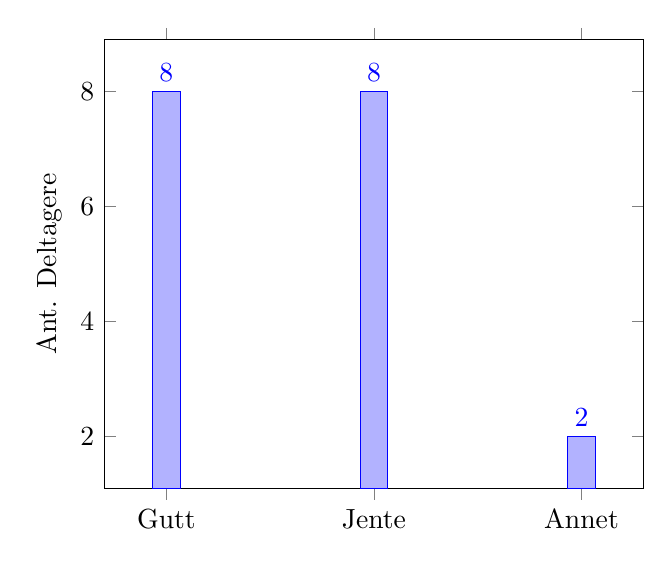
\begin{tikzpicture}
        \begin{axis}[ybar, enlargelimits=0.15, legend style={at={(0.5,-0.2)},
            anchor=north, legend columns=-1}, ylabel={Ant. Deltagere},
            symbolic x coords={Gutt, Jente, Annet}, xtick=data,
            nodes near coords, nodes near coords align={vertical},]
            % x tick label style={rotate=15, anchor=east},]
            \addplot coordinates {(Gutt, 8) (Jente, 8) (Annet, 2)};
        \end{axis}
    \end{tikzpicture}
    \caption{Test}
\end{figure}

\newpage